\subsection{Convolutional Neural Networks}\label{sec:cnn}

There are a couple of glaring problems with neural network layers as they were introduced in section \ref{sec:ANN}. Firstly they are hardly efficient either by memory or by flops, secondly there is the question of invariance. Developed primarily for images convolutional neural networks aims at increasing both efficiency and modeling power when faced with data that has some translational symmetry. For image-data this is intuitively a strong assumption since the object of interest can have many different positions on the canvas and still be the same object. However convolutional neural networks do not address the two other evident symmetries for image data; rotation and scale. In short the advantage of convolutional layers is an allowance for a vastly reduced number of parameters if there is some translational symmetry in the data at the cost of much higher demands of memory. The convolutional forward pass is illustrated in figure \ref{fig:conv_aritmetic}. A $n\times n$ kernel, a matrix of weights, is convolved with the input image by taking the inner product with a $n\times n$ patch of the image iteratively moving over the entire input. The convolution is computed over the entire depth of the input, i.e. along the channels of the image. Thus the kernel maintains a $n\times n$ matrix of weights for each layer of depth in the previous layer. For a square kernel that moves one pixel from left to right per step over a square image the output is then a square matrix with size as defined in equation \ref{eq:simple_conv_out} for each filter. 

\begin{equation}\label{eq:simple_conv_out}
O = W - K +1
\end{equation}

\noindent Where $W$ is the width/height of the input and $K$ the width/height of the kernel. In practice, however, it is beneficial to pad the image with one or more columns/rows of zeros such that the kernel fully covers the input. Additionally one can down-sample by moving the kernel more than one pixel at a time, this is called the stride of the layer. The full computation of the down-sizing with these effects then is a modified version of equation \ref{eq:simple_conv_out}, namely: 

\begin{equation}\label{eq:conv_out}
O = \frac{W - K + 2P}{S} + 1
\end{equation} 

\noindent The modification includes the addition of an additive term from the padding, $P$, and a division by the stride (i.e. how many pixels the kernel jumps each step), $S$. Striding provides a convenient way to down-sample the input which lessens the memory needed to train the model. Traditionally MaxPooling has also been used to achieve the same result. MaxPooling is a naive down-sampling algorithm that simply selects the highest value from the set of disjoint $m\times m$ patches of the input. Where $m$ is the pooling number, and we note that $m=2$ results in a halving of the input in both width and height. \todo{Include mathematical formulation of the convolutional layer}
\begin{figure}
\centering
\subfloat[{}]{{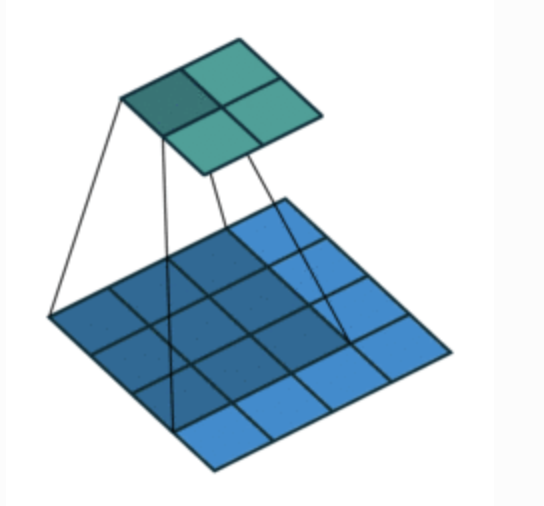
\includegraphics[width=0.5\textwidth]{../figures/conv_illustration}}}
\subfloat[{}]{{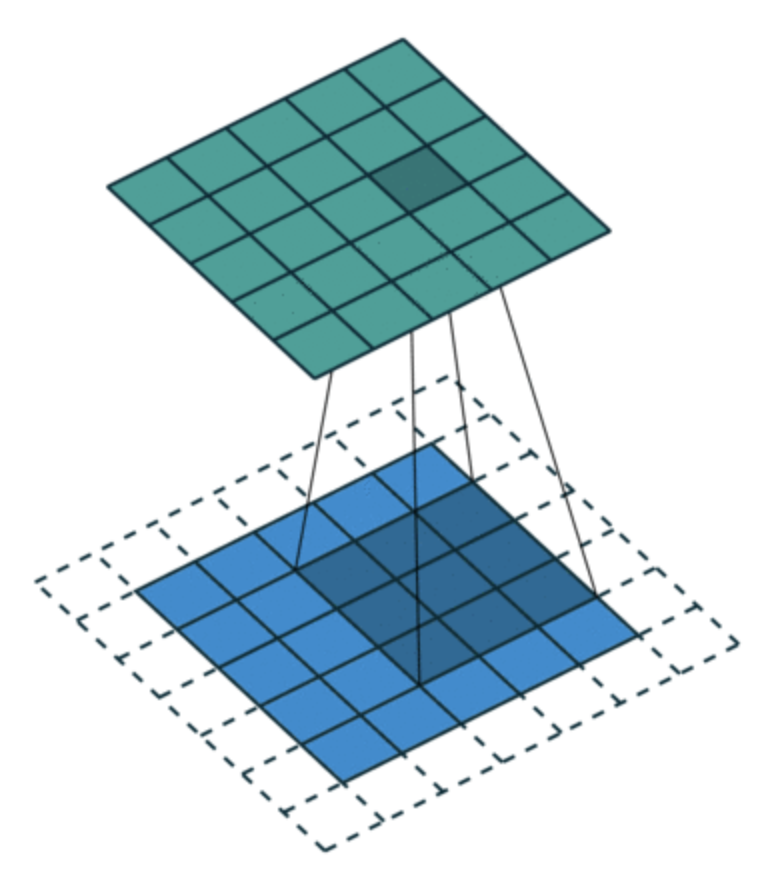
\includegraphics[width=0.5\textwidth]{../figures/conv_zeropad_illustration}}}
\caption[Convolutional layer illustration]{Two examples of a convolutional layers forward pass, which is entirely analogous to equation \ref{eq:fwd_multi} for fully connected layers. The convolutional layer maintains a $N$ kernels, or filters, that slides over the input taking the dot product for each step, this is the convolution of the kernel with the input. In \textbf{(a)} a $3\times3$ kernel is at the first position of the input and produces one floating point output for the $9$ pixels it sees. The kernel is a matrix of weights that are updated with backpropagation of errors. An obvious problem with \textbf{(a)} is that the kernel center cannot be placed at the edges of the image, we solve this by padding the image with zeros along the outer edges. This zero-padding is illustrated in \textbf{b} where zeros are illustrated by the dashed lines surrounding the image. The kernel then convolves over the whole image including the zeroed regions thus loosing less information. Figure copied from \citet{Dumoulin2016}}\label{fig:conv_aritmetic} 
\end{figure}

\begin{figure}
\centering
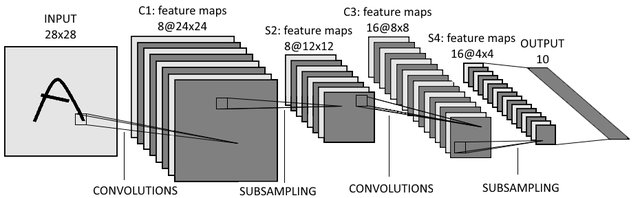
\includegraphics[width=\textwidth]{../figures/lenet5}
\caption[Original LeNet architecture]{The architecture \citet{Lecun1998} used when introducing convolutional layers. Each convolutional layer maintains $N$ kernels with initially randomized weights. These $N$ filters act on the same input, but will extract different features from the input owing to their random initialization. The output from a convolutional layer then has size determined by equation \ref{eq:conv_out} multiplied by the number of filters $N$. Every $t$-th layer will down-sample the input, usually by a factor two. Either by striding the convolution or by MaxPooling.}\label{fig:lenet5}
\end{figure}

Originally proposed by \citet{Lecun1998} convolutional layers were used as feature extractors, i.e. to recognize and extract parts of images that could be fed to ordinary fully connected layers. The use of convolutional layers remained in partial obscurity for largely computational reasons until the rise to preeminence when Alex Krizhevsky et. al won a major image recognition contest in 2012 (\cite{Krizhevsky2012}) using connected graphical processing units (GPUs). A GPU is a specialized device constructed to write data to display to a computer screen. This involves large matrix-multiplications which is what Krizhevsky et. al abused to achieve the entrance of convolutional networks truly to the main-stage of machine learning. 

Since then there have been major revolutions in architecture for the state-of-the-art. Inception modules showed that combinations of filters are functionally the same as ones with larger kernels yet maintain fewer parameters (\cite{Szegedy2014}). Residual networks used skip connections, passing the original data forward to avoid vanishing graadients, and batch normalization (discussed in section \ref{sec:batchnorm}). In this thesis however, the number of classes and amount of data is still far less complex than the cases where these technologies have really shown their worth\footnote{The AT-TPC produces data on the order of $10^5$ datapoints and $10^0$ classes while inception-net and residual nets deal with datasets on the order of millions and $10^3$ classes}.

\subsubsection{A small digression on GPUs}
Usually these devices are used in expensive video operations such as those required for visual effects and video games. They are specialized in processing large matrix operations which is exactly the kind of computational resource neural networks profit from. The major bottle-neck they had to solve was the problem of memory, at the time a GPU only had about $3 GB$ of memory. They were however well equipped to communicate without writing to the central system memory so the authors ended up implementing an impressive load-sharing paradigm (\cite{Krizhevsky2012}). Modern consumer grade GPUs have up to $10 GB$ of memory and have more advanced sharing protocols further cementing them as ubiquitous in machine learning research. In this thesis all models were run on high-end consumer grade GPUs hosted by the AI-HUB computational resource at UIO.

